% Options for packages loaded elsewhere
\PassOptionsToPackage{unicode}{hyperref}
\PassOptionsToPackage{hyphens}{url}
%
\documentclass[
]{article}
\usepackage{amsmath,amssymb}
\usepackage{iftex}
\ifPDFTeX
  \usepackage[T1]{fontenc}
  \usepackage[utf8]{inputenc}
  \usepackage{textcomp} % provide euro and other symbols
\else % if luatex or xetex
  \usepackage{unicode-math} % this also loads fontspec
  \defaultfontfeatures{Scale=MatchLowercase}
  \defaultfontfeatures[\rmfamily]{Ligatures=TeX,Scale=1}
\fi
\usepackage{lmodern}
\ifPDFTeX\else
  % xetex/luatex font selection
\fi
% Use upquote if available, for straight quotes in verbatim environments
\IfFileExists{upquote.sty}{\usepackage{upquote}}{}
\IfFileExists{microtype.sty}{% use microtype if available
  \usepackage[]{microtype}
  \UseMicrotypeSet[protrusion]{basicmath} % disable protrusion for tt fonts
}{}
\makeatletter
\@ifundefined{KOMAClassName}{% if non-KOMA class
  \IfFileExists{parskip.sty}{%
    \usepackage{parskip}
  }{% else
    \setlength{\parindent}{0pt}
    \setlength{\parskip}{6pt plus 2pt minus 1pt}}
}{% if KOMA class
  \KOMAoptions{parskip=half}}
\makeatother
\usepackage{xcolor}
\usepackage[margin=1in]{geometry}
\usepackage{color}
\usepackage{fancyvrb}
\newcommand{\VerbBar}{|}
\newcommand{\VERB}{\Verb[commandchars=\\\{\}]}
\DefineVerbatimEnvironment{Highlighting}{Verbatim}{commandchars=\\\{\}}
% Add ',fontsize=\small' for more characters per line
\usepackage{framed}
\definecolor{shadecolor}{RGB}{248,248,248}
\newenvironment{Shaded}{\begin{snugshade}}{\end{snugshade}}
\newcommand{\AlertTok}[1]{\textcolor[rgb]{0.94,0.16,0.16}{#1}}
\newcommand{\AnnotationTok}[1]{\textcolor[rgb]{0.56,0.35,0.01}{\textbf{\textit{#1}}}}
\newcommand{\AttributeTok}[1]{\textcolor[rgb]{0.13,0.29,0.53}{#1}}
\newcommand{\BaseNTok}[1]{\textcolor[rgb]{0.00,0.00,0.81}{#1}}
\newcommand{\BuiltInTok}[1]{#1}
\newcommand{\CharTok}[1]{\textcolor[rgb]{0.31,0.60,0.02}{#1}}
\newcommand{\CommentTok}[1]{\textcolor[rgb]{0.56,0.35,0.01}{\textit{#1}}}
\newcommand{\CommentVarTok}[1]{\textcolor[rgb]{0.56,0.35,0.01}{\textbf{\textit{#1}}}}
\newcommand{\ConstantTok}[1]{\textcolor[rgb]{0.56,0.35,0.01}{#1}}
\newcommand{\ControlFlowTok}[1]{\textcolor[rgb]{0.13,0.29,0.53}{\textbf{#1}}}
\newcommand{\DataTypeTok}[1]{\textcolor[rgb]{0.13,0.29,0.53}{#1}}
\newcommand{\DecValTok}[1]{\textcolor[rgb]{0.00,0.00,0.81}{#1}}
\newcommand{\DocumentationTok}[1]{\textcolor[rgb]{0.56,0.35,0.01}{\textbf{\textit{#1}}}}
\newcommand{\ErrorTok}[1]{\textcolor[rgb]{0.64,0.00,0.00}{\textbf{#1}}}
\newcommand{\ExtensionTok}[1]{#1}
\newcommand{\FloatTok}[1]{\textcolor[rgb]{0.00,0.00,0.81}{#1}}
\newcommand{\FunctionTok}[1]{\textcolor[rgb]{0.13,0.29,0.53}{\textbf{#1}}}
\newcommand{\ImportTok}[1]{#1}
\newcommand{\InformationTok}[1]{\textcolor[rgb]{0.56,0.35,0.01}{\textbf{\textit{#1}}}}
\newcommand{\KeywordTok}[1]{\textcolor[rgb]{0.13,0.29,0.53}{\textbf{#1}}}
\newcommand{\NormalTok}[1]{#1}
\newcommand{\OperatorTok}[1]{\textcolor[rgb]{0.81,0.36,0.00}{\textbf{#1}}}
\newcommand{\OtherTok}[1]{\textcolor[rgb]{0.56,0.35,0.01}{#1}}
\newcommand{\PreprocessorTok}[1]{\textcolor[rgb]{0.56,0.35,0.01}{\textit{#1}}}
\newcommand{\RegionMarkerTok}[1]{#1}
\newcommand{\SpecialCharTok}[1]{\textcolor[rgb]{0.81,0.36,0.00}{\textbf{#1}}}
\newcommand{\SpecialStringTok}[1]{\textcolor[rgb]{0.31,0.60,0.02}{#1}}
\newcommand{\StringTok}[1]{\textcolor[rgb]{0.31,0.60,0.02}{#1}}
\newcommand{\VariableTok}[1]{\textcolor[rgb]{0.00,0.00,0.00}{#1}}
\newcommand{\VerbatimStringTok}[1]{\textcolor[rgb]{0.31,0.60,0.02}{#1}}
\newcommand{\WarningTok}[1]{\textcolor[rgb]{0.56,0.35,0.01}{\textbf{\textit{#1}}}}
\usepackage{graphicx}
\makeatletter
\newsavebox\pandoc@box
\newcommand*\pandocbounded[1]{% scales image to fit in text height/width
  \sbox\pandoc@box{#1}%
  \Gscale@div\@tempa{\textheight}{\dimexpr\ht\pandoc@box+\dp\pandoc@box\relax}%
  \Gscale@div\@tempb{\linewidth}{\wd\pandoc@box}%
  \ifdim\@tempb\p@<\@tempa\p@\let\@tempa\@tempb\fi% select the smaller of both
  \ifdim\@tempa\p@<\p@\scalebox{\@tempa}{\usebox\pandoc@box}%
  \else\usebox{\pandoc@box}%
  \fi%
}
% Set default figure placement to htbp
\def\fps@figure{htbp}
\makeatother
\setlength{\emergencystretch}{3em} % prevent overfull lines
\providecommand{\tightlist}{%
  \setlength{\itemsep}{0pt}\setlength{\parskip}{0pt}}
\setcounter{secnumdepth}{-\maxdimen} % remove section numbering
\usepackage{bookmark}
\IfFileExists{xurl.sty}{\usepackage{xurl}}{} % add URL line breaks if available
\urlstyle{same}
\hypersetup{
  hidelinks,
  pdfcreator={LaTeX via pandoc}}

\author{}
\date{\vspace{-2.5em}}

\begin{document}

\subsection{Anova Example 1}\label{anova-example-1}

\subsubsection{Plot the Data}\label{plot-the-data}

\begin{Shaded}
\begin{Highlighting}[]
\FunctionTok{suppressMessages}\NormalTok{(}\FunctionTok{library}\NormalTok{(ggplot2))}
\NormalTok{mlb }\OtherTok{\textless{}{-}} \FunctionTok{read.csv}\NormalTok{(}\StringTok{"https://raw.githubusercontent.com/roualdes/data/master/mlb.csv"}\NormalTok{)}
\NormalTok{p }\OtherTok{\textless{}{-}} \FunctionTok{ggplot}\NormalTok{(}\AttributeTok{data=}\NormalTok{mlb, }\FunctionTok{aes}\NormalTok{(}\AttributeTok{x=}\NormalTok{position, }\AttributeTok{y=}\NormalTok{salary)) }\SpecialCharTok{+}
\FunctionTok{geom\_boxplot}\NormalTok{() }\SpecialCharTok{+}
\FunctionTok{theme}\NormalTok{(}\AttributeTok{axis.text.x=}\FunctionTok{element\_text}\NormalTok{(}\AttributeTok{angle=}\DecValTok{45}\NormalTok{, }\AttributeTok{hjust=}\DecValTok{1}\NormalTok{))}
\NormalTok{p}
\end{Highlighting}
\end{Shaded}

\pandocbounded{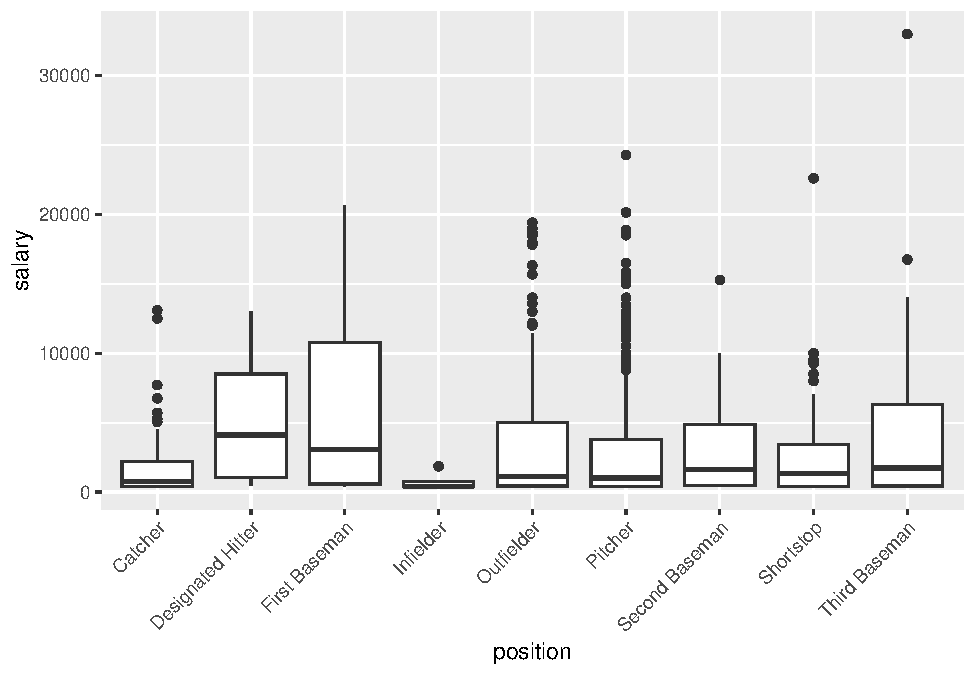
\includegraphics[keepaspectratio]{2025-11-12-anova_files/figure-latex/unnamed-chunk-1-1.pdf}}

\subsubsection{Linear Model}\label{linear-model}

The \texttt{lm} function creates a fitted linear model from the given
variables and data set.

The \texttt{anova} function performs analysis of variance on the
resulting linear model object

\begin{Shaded}
\begin{Highlighting}[]
\NormalTok{model }\OtherTok{\textless{}{-}} \FunctionTok{lm}\NormalTok{(salary}\SpecialCharTok{\textasciitilde{}}\NormalTok{position, }\AttributeTok{data=}\NormalTok{mlb)}
\NormalTok{model}
\end{Highlighting}
\end{Shaded}

\begin{verbatim}
## 
## Call:
## lm(formula = salary ~ position, data = mlb)
## 
## Coefficients:
##               (Intercept)  positionDesignated Hitter  
##                    1937.2                     3298.5  
##     positionFirst Baseman          positionInfielder  
##                    3889.3                    -1166.6  
##        positionOutfielder            positionPitcher  
##                    1816.7                     1062.0  
##    positionSecond Baseman          positionShortstop  
##                    1085.5                      906.9  
##     positionThird Baseman  
##                    2704.1
\end{verbatim}

\begin{Shaded}
\begin{Highlighting}[]
\NormalTok{res }\OtherTok{\textless{}{-}} \FunctionTok{anova}\NormalTok{(model)}
\NormalTok{res}
\end{Highlighting}
\end{Shaded}

\begin{verbatim}
## Analysis of Variance Table
## 
## Response: salary
##            Df     Sum Sq  Mean Sq F value    Pr(>F)    
## position    8 6.0975e+08 76219146  3.9307 0.0001422 ***
## Residuals 819 1.5881e+10 19390502                      
## ---
## Signif. codes:  0 '***' 0.001 '**' 0.01 '*' 0.05 '.' 0.1 ' ' 1
\end{verbatim}

\begin{Shaded}
\begin{Highlighting}[]
\CommentTok{\# Ensure that the position variable is a factor}
\FunctionTok{is.factor}\NormalTok{(mlb[,}\StringTok{"position"}\NormalTok{])}
\end{Highlighting}
\end{Shaded}

\begin{verbatim}
## [1] FALSE
\end{verbatim}

\begin{Shaded}
\begin{Highlighting}[]
\NormalTok{alpha }\OtherTok{\textless{}{-}} \FloatTok{0.05}

\NormalTok{res}\SpecialCharTok{$}\StringTok{"Pr(\textgreater{}F)"}\NormalTok{[}\DecValTok{1}\NormalTok{] }\SpecialCharTok{\textless{}}\NormalTok{ alpha}
\end{Highlighting}
\end{Shaded}

\begin{verbatim}
## [1] TRUE
\end{verbatim}

Because p-value is less than \(alpha\)=0.05, we reject the null
hypothesis.

\subsection{Anova Example 2: Carnivora}\label{anova-example-2-carnivora}

\subsubsection{Obtain Data}\label{obtain-data}

\begin{Shaded}
\begin{Highlighting}[]
\FunctionTok{suppressMessages}\NormalTok{(\{}\FunctionTok{library}\NormalTok{(ape)}
\FunctionTok{library}\NormalTok{(dplyr)}
\FunctionTok{library}\NormalTok{(ggplot2)}
\FunctionTok{data}\NormalTok{(carnivora)\})}
\end{Highlighting}
\end{Shaded}

\begin{Shaded}
\begin{Highlighting}[]
\CommentTok{\# Filter down to just 5 families}

\FunctionTok{data}\NormalTok{(carnivora)}

\CommentTok{\# Remove 3 families}
\NormalTok{carnivs }\OtherTok{\textless{}{-}} \FunctionTok{filter}\NormalTok{(carnivora,}
\SpecialCharTok{!}\NormalTok{(Family }\SpecialCharTok{\%in\%} \FunctionTok{c}\NormalTok{(}\StringTok{"Ailuridae"}\NormalTok{,}
\StringTok{"Procyonidae"}\NormalTok{,}
\StringTok{"Viverridae"}\NormalTok{)))}
\FunctionTok{head}\NormalTok{(carnivs)}
\end{Highlighting}
\end{Shaded}

\begin{verbatim}
##       Order SuperFamily  Family  Genus         Species   FW   SW    FB    SB
## 1 Carnivora  Caniformia Canidae  Canis     Canis lupus 31.1 33.1 130.0 132.3
## 2 Carnivora  Caniformia Canidae  Canis   Canis latrans  9.7 10.6  84.5  88.3
## 3 Carnivora  Caniformia Canidae  Canis   Canis adustus 10.6 11.3  53.5  51.8
## 4 Carnivora  Caniformia Canidae  Canis Canis mesomelas  7.2  7.7  52.0  56.8
## 5 Carnivora  Caniformia Canidae Lycaon   Lycaon pictus 22.2 22.0 128.0 129.0
## 6 Carnivora  Caniformia Canidae   Cuon    Cuon alpinus 13.8 15.8  95.0  95.0
##    LS   GL  BW WA  AI  LY    AM IB
## 1 5.5 63.0 425 35  NA 177   913 12
## 2 6.2 61.5 225 98  NA  NA   365 12
## 3 4.3 63.3  NA NA  NA 127         
## 4 3.8 60.0  NA 61 270  NA   392   
## 5 8.8 70.5 365 77 390 132 t 132 13
## 6 4.3 62.0 275 NA  NA 186
\end{verbatim}

\begin{Shaded}
\begin{Highlighting}[]
\CommentTok{\# Run anova}
\NormalTok{mod }\OtherTok{\textless{}{-}} \FunctionTok{lm}\NormalTok{(SB}\SpecialCharTok{\textasciitilde{}}\NormalTok{Family, }\AttributeTok{data=}\NormalTok{carnivs)}
\FunctionTok{anova}\NormalTok{(mod)}
\end{Highlighting}
\end{Shaded}

\begin{verbatim}
## Analysis of Variance Table
## 
## Response: SB
##           Df Sum Sq Mean Sq F value    Pr(>F)    
## Family     4 354999   88750  37.333 < 2.2e-16 ***
## Residuals 70 166406    2377                      
## ---
## Signif. codes:  0 '***' 0.001 '**' 0.01 '*' 0.05 '.' 0.1 ' ' 1
\end{verbatim}

\subsubsection{Plot the Data}\label{plot-the-data-1}

\begin{Shaded}
\begin{Highlighting}[]
\NormalTok{p }\OtherTok{\textless{}{-}} \FunctionTok{ggplot}\NormalTok{(carnivs, }\FunctionTok{aes}\NormalTok{(Family, SB)) }\SpecialCharTok{+}
\FunctionTok{geom\_point}\NormalTok{() }\SpecialCharTok{+}
\FunctionTok{stat\_summary}\NormalTok{(}\AttributeTok{fun=}\NormalTok{mean, }\AttributeTok{colour=}\StringTok{"red"}\NormalTok{,}
\AttributeTok{geom=}\StringTok{"point"}\NormalTok{, }\AttributeTok{size=}\DecValTok{4}\NormalTok{) }\SpecialCharTok{+}
\FunctionTok{labs}\NormalTok{(}\AttributeTok{y=}\StringTok{"Brain Weight"}\NormalTok{)}
\NormalTok{p}
\end{Highlighting}
\end{Shaded}

\pandocbounded{\includegraphics[keepaspectratio]{2025-11-12-anova_files/figure-latex/unnamed-chunk-7-1.pdf}}

\subsubsection{Coefficients}\label{coefficients}

Calling the function \texttt{coefficients} on the linear model returns
the intercept and \(k − 1\) values \(\beta_j\)

\begin{Shaded}
\begin{Highlighting}[]
\FunctionTok{coefficients}\NormalTok{(mod)}
\end{Highlighting}
\end{Shaded}

\begin{verbatim}
##      (Intercept)    FamilyFelidae  FamilyHyaenidae FamilyMustelidae 
##         59.45556         28.14444         36.44444        -29.47056 
##    FamilyUrsidae 
##        282.86944
\end{verbatim}

\begin{Shaded}
\begin{Highlighting}[]
\CommentTok{\# Compare coefficients to group means}
\NormalTok{carnivs }\SpecialCharTok{\%\textgreater{}\%}
    \FunctionTok{group\_by}\NormalTok{(Family) }\SpecialCharTok{\%\textgreater{}\%}
    \FunctionTok{summarise}\NormalTok{(}\AttributeTok{m=}\FunctionTok{mean}\NormalTok{(SB))}
\end{Highlighting}
\end{Shaded}

\begin{verbatim}
## # A tibble: 5 x 2
##   Family         m
##   <fct>      <dbl>
## 1 Canidae     59.5
## 2 Felidae     87.6
## 3 Hyaenidae   95.9
## 4 Mustelidae  30.0
## 5 Ursidae    342.
\end{verbatim}

\begin{Shaded}
\begin{Highlighting}[]
\CommentTok{\# Retriece fitted values}
\NormalTok{yhat }\OtherTok{\textless{}{-}} \FunctionTok{fitted}\NormalTok{(mod)}
\FunctionTok{head}\NormalTok{(yhat)}
\end{Highlighting}
\end{Shaded}

\begin{verbatim}
##        1        2        3        4        5        6 
## 59.45556 59.45556 59.45556 59.45556 59.45556 59.45556
\end{verbatim}

\begin{Shaded}
\begin{Highlighting}[]
\FunctionTok{tail}\NormalTok{(yhat)}
\end{Highlighting}
\end{Shaded}

\begin{verbatim}
##   70   71   72   73   74   75 
## 87.6 87.6 87.6 87.6 87.6 87.6
\end{verbatim}

\end{document}
